\chapter{Overall Description}

\section{Product Perspective}

\acrshort{csaf} serves the role of a middleware for closed loop system simulations. A user starts with a model that they have for a system, with well-defined inputs, outputs and states. Shown in Figure \ref{fig:ccomp}, they will proceed to create a \acrshort{csaf} pub/sub component. The package comes with an \acrshort{api} to make common system descriptions easy to implement, and has a wrappers if the system is a black box. 
The component is described using a small configuration file, and can be interacted with using a subscriber and a publisher. The pub/sub pair is for temporal input and output---input can be specified at a given time in order to receive output at the specified time. \\

\begin{figure}
\centering
\includegraphics[width=0.9\textwidth]{componentcomposition.pdf}
\caption{Structure of a CSAF Compatible Component}
\label{fig:ccomp}
\end{figure}

These CSAF components can be composed together to create a closed loop system. Figure \ref{fig:csys} shows the blocks composed under a system analyzer. In the scope of controls research, analyses can be created and performed on the modular CSAF components. \\

\begin{figure}
\centering
\includegraphics[width=0.9\textwidth]{systemanalysis.pdf}
\caption{A closed loop system represented as pub/sub components. Control signals are broadcasted as a collection of messages with specific topics. The component processes the input, producing system output as a collection of messages with topics. }
\label{fig:csys}
\end{figure}


\section{Product Functions}

A user is able to

\begin{enumerate}
\item add model specifics of a dynamical system to create a compatible component
\item compose controllers together to make closed loop systems
\item simulate a closed loop systems efficiently
\item design custom analyses, and is supported with libraries and documentation
\end{enumerate}

Figure \ref{fig:uworkflow} shows the user workflow for a systems analysis, from start to finish. All blocks in the control diagram must exist as components. Then, the components are composed together to achieve the controlled system. The system is ready to be simulated or analyzed.

\begin{figure}
\centering
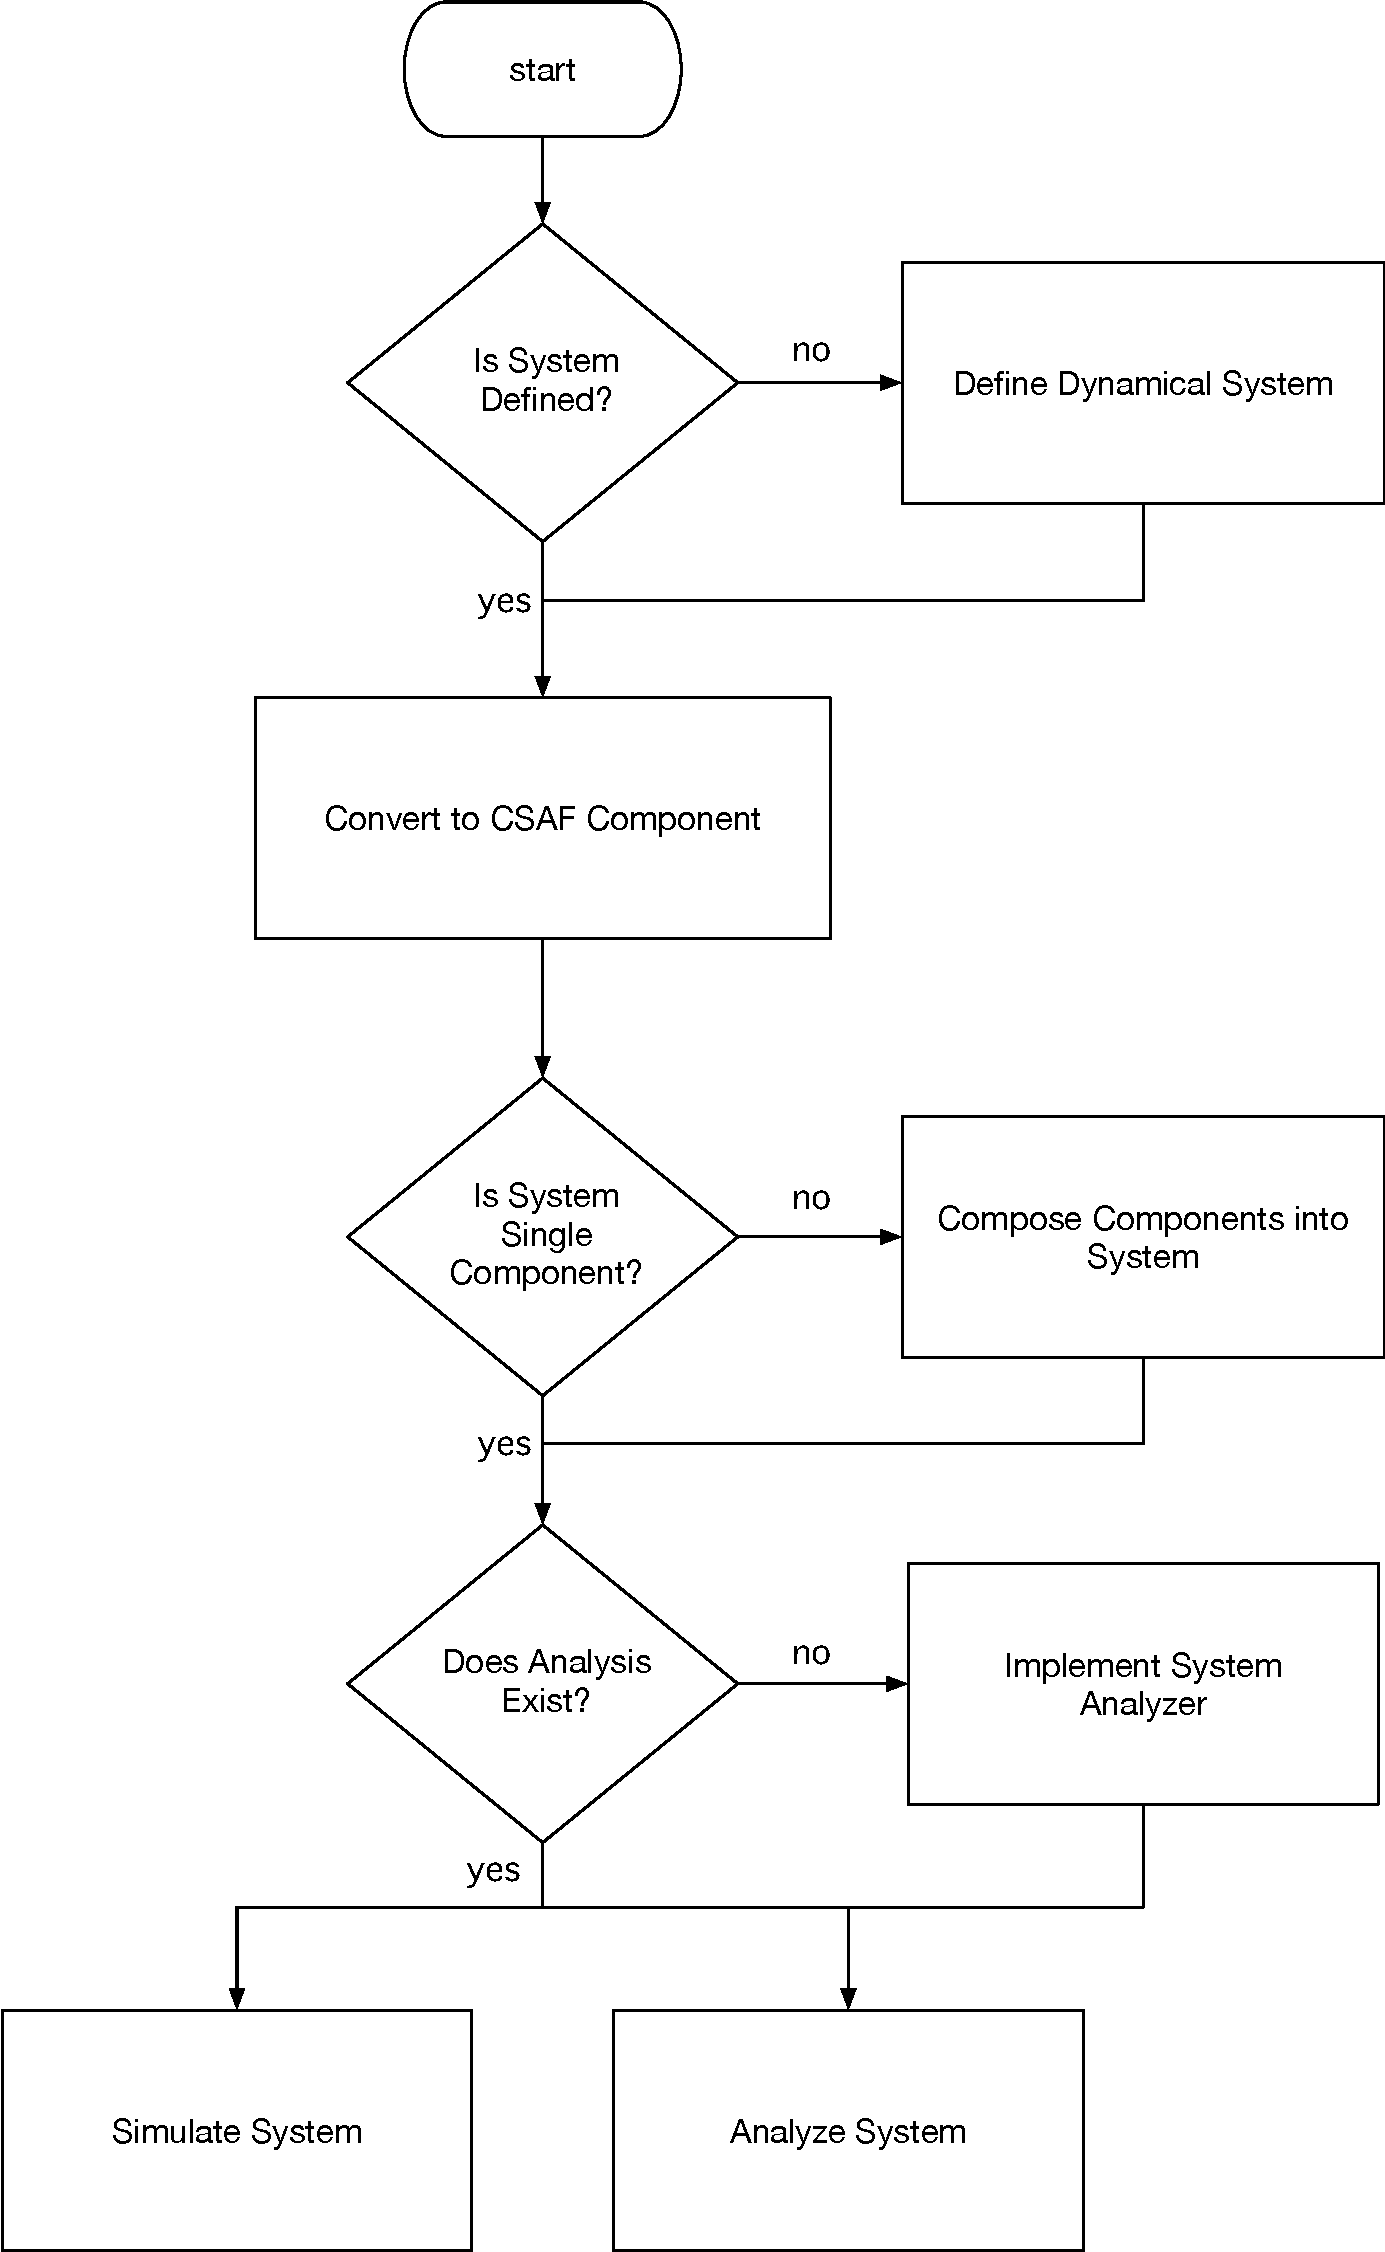
\includegraphics[width=0.85\textwidth]{userworkflow2.pdf}
\caption{ \acrshort{csaf} System Analysis User Workflow }
\label{fig:uworkflow}
\end{figure}

\section{User Classes and Characteristics}

\acrshort{csaf}'s user workflow is restricted to software developers, systems engineers and researchers. The users implementing components are required to have knowledge of programming and system theory. The workflow output is to provide results for a controls research project. As such, secondary users are project managers and reviewers. 


\section{Operating Environment}

\acrshort{csaf} is implemented in modern python (3.5+), with specific packages for numerical/controls 
computing. Also, it has optional package requirements, like Tensorflow and RosPy needed for specific 
features. Its primary use is to operate inside a debian based docker container for its delivery in the 
\acrlong{aa} project, as well be shipped inside of a virtual machine. For full use, it will require a OS with 
CoPilot installed, needing Haskell and C toolchains.  

\section{Design and Implementation Constraints}

\acrshort{csaf} is requested to support integration with deliverables from other teams in the \acrshort{aa} 
project; it is required to create and accept \acrshort{ros} messages as a serialization method to be 
compatible with external systems. For visualization, the ability to communicate with FlightGear is requested 
to make visualization of aircraft systems possible. \\

\section{User Documentation}

As \acrshort{csaf} users will need detailed knowledge of its architecture and \acrshort{api} to use it 
effectively, documentation is important. Its code repository contain a number of markdown files that outline 
the installation and setup. For object and function level documentation, the code uses an ample amount of 
Python docstrings, which can be used to autogenerate \acrshort{api} documentation provided the code 
comments are suitably detailed. \\

\acrshort{api} level documentation is not enough, and a user manual is available. This manual is conscience 
of task oriented documentation; the workflow is discussed and examples are provided for intended 
implementation use. Further, the use cases are also described in Jupyter notebooks, which provide an 
interactive platform to experiment with code.

\section{Assumptions and Dependencies}

\acrshort{csaf}'s middleware approach can add substantial overhead to processing a closed loop system, as 
the serialization, transportation and deserialization over sockets can be much slower than doing everything in 
one application. The target system is assumed to have relatively low frequency sampling rates or short time 
span. If a multi-timescale system is added, the time domain simulation approach can be inefficient. If such a 
system were of interest in the \acrshort{aa} project, new simulation methods may need to be investigated.\\

\subsection{Limitations}

No planned support for
\begin{enumerate}
\item closed loop continuous time controllers
\item interaction with fast/time critical systems
\end{enumerate}
